\documentclass[onecolumn,preprintnumbers,amsmath,amssymb,superscriptaddress]{revtex4}
%\usepackage[pdftex]{graphicx}

\usepackage{amsmath,amsfonts,amssymb}
\usepackage[english]{babel}
\usepackage[latin1]{inputenc}
\usepackage[T1]{fontenc}
\usepackage{color}
\usepackage{float}
\usepackage{verbatim}
\usepackage{graphicx}
\usepackage{bm}
\usepackage{mathtools}
\usepackage{stmaryrd}
\usepackage{anyfontsize}
\usepackage{color}
%\usepackage{lineno}
%\usepackage[left]{lineno}
%\usepackage[comma,sort&compress]{natbib}

%\bibliographystyle{ieeetr}


%\linenumbers
%\setlength\linenumbersep{3pt}

\begin{document}

% \author{Taran Rallings} \affiliation{School of Natural Sciences, University
%   of California, Merced, Merced, CA 95340, USA}

% \author{Kevin Uno} \affiliation{Lamont Doherty Earth Observatory}

% \author{Justin D. Yeakel} \affiliation{School of Natural Sciences, University
%   of California, Merced, Merced, CA 95340, USA}


\title{Predation mortality allometries}

\maketitle

\section*{Predator mortality rate}

We next explore the effect of predator mortality on an herbivore population, taking into account carnivore-specific growth and energetic rates.
Without explicitely taking into account the dynamics of a predator population, we can account for the effects of an implicit predator $P$ with mass $M_P$ on the population of the consumer $C$ with mass $M_C$, where we will for now assume that the predator population exists at some steady state $P^*$.
The effect of the predator on the consumer's population is given by
\begin{align}
\frac{\rm d}{\rm dt}C &= -bP^*C, \nonumber \\
	b &= \frac{\lambda_{\rm P}}{Y_P k_C^{\rm max}},
\end{align}
where $b$ is the capture efficiency of the predator on the consumer, $P^*$ is the steady state density of the predator population, $\lambda_P$ is the maximum growth rate of the predator, $k_C^{\rm max}$ is the density of the consumer population that maximizes this predator growth, and $Y_P$ is the yield coefficent for the predator.
As we are not tracking ${\rm d}P/{\rm dt}$, we assume a constant predator population density given by Damuth's Law, but where the slope and intercept consider only measured densities of predatory mammals.
If $P$ is g/m${}^2$, the density of individuals/m${}^2$ then follows $(1/M_P)P^*(M_P) \propto M_P^{-0.88}$. 


The predator's yield $Y_P$ is calculated
\begin{equation}
Y_P = \frac{M_P E_C}{\int_0^{t_{\lambda_P}}B_0^Pm_P(t)^\eta {\rm dt}},
\end{equation}
where $m_P(t)$ is the ontogenetic mass of an individual predator as it grows over time to an adult mass $M_P$.
The parameters $t_{\lambda_P}$ and $B_0^P$ are the timescale associated with reaching reproductive maturity and the metabolic coefficient for predatory mammals, respectively, and $\eta=-3/4$ is the metabolic exponent.
In words, the predator yield scales proportionally with the individual mass of the predator (g) and the energy density of prey $E_C$ (J/g), normalized to the lifetime energetic needs of a predator reaching maturity (J).
Accordingly, the predator yield coefficient describes the grams of predator produced per gram of prey consumed.

We assume that predators consume all non-skeletal mass of prey. 
Because the amount of consumable tissues with different energy densities within an herbivore varies allometrically, so too should the energy density $E_C$.
We consider four primary tissue groups: a consumable set composed of muscle, fat, and \emph{other} tissues, and an non-consumable set composed only of skeletal tissues.
If the scalings associated with fat, muscle, and skeletal tissues are $M_C^{\rm fat}=f_0 M_C^{1.19}$, $M_C^{\rm musc} = g_0 M_C^{1.00}$, and $M_C^{\rm skel} = h_0 M_C^{1.09}$, the scaling of the \emph{other} tissue (gut tissue, organ tissue, etc) is given by $M_C^{\rm other} = M_C - (M_C^{\rm fat} + M_C^{\rm musc} + M_C^{\rm skel})$.
The energy density of fat is $E_{\rm fat} = 37700$ J/g, whereas the energy density of muscle is $E_{\rm musc} = 17900$ J/g.
If we assume that gut and organ tissues have roughly the same energy density as muscle, the attainable energy density for an herbivore of size $M_C$ is given by
\begin{equation}
	E_C(M_C) = E_{\rm fat}\frac{M_C^{\rm fat}}{M_C} + E_{\rm musc}\left(\frac{M_C^{\rm musc}}{M_C} + \frac{M_C^{\rm other}}{M_C} \right).
\end{equation}

Another important consideration is that we have assigned $k_C^{\rm max}$ to represent the consumer density maximizing predator growth $\lambda_P$.
Because predator growth is proportional to prey growth, and prey growth is responding to a logistically growing resource $R$, we assume that predator growth is maximized when prey growth is maximized, which occurs when the resource reaches its half-saturation point $R = k_R/2$ g/m${}^2$, where we assume $k_R = 23000$ g/m${}^2$.
The translated available consumer biomass represented by this half-saturation point is then given by $k_C^{\rm max} = Y_C k_R/2$ (consumer g/m${}^2$) where $Y_C$ is the consumer yield coefficient, giving the grams of consumer per grams of resource and calculated analagously to $Y_P$, such that
\begin{equation}
	Y_C = \frac{M_C E_R}{\int_0^{t_{\lambda_C}}B_0^C m_C(t)^\eta {\rm dt}},
\end{equation}
where $m_C(t)$ is the ontogenetic mass of an individual herbivorous consumer as it grows over time to an adult mass $M_C$.
The parameters $t_{\lambda_C}$ and $B_0^C$ are the timescale associated with reaching reproductive maturity and the metabolic coefficient for herbivorous mammals, respectively, and $\eta=-3/4$ is the metabolic exponent.
Moreover, we assume a resource energy density that approximates graze, such that $E_R = 18200$ J/g.

Because predator-prey relationships tend to be determined largely by the body sizes of predator and prey, the mortality of a prey consumer due to predation requires us to assume a consumer with mass $M_C$ has a predator with body mass $M_P$.
The probability of a trophic interaction between predators and prey $\ell_{C,P}$ as a function of the body sizes of both follows a logit relationship, where
\begin{equation}
	\log \left(\frac{Pr(\ell_{C,P})=1}{Pr(\ell_{C,P})=0}\right) = q_0 + q_1 \log \left(\frac{M_C}{M_P}\right) + q_2 \log^2\left(\frac{M_C}{M_P}\right).
\end{equation}
and the parameters ${\bm q} = (q_0,q_1,q_2)$ are fitted to an adjacency matrix describing empirical interactions between predators and prey of different body sizes within a community. 
The result for diverse terrestrial mammalian communities such as that in the Serengeti results in a Guassian-shaped distribution in log body mass space, where for a particular predator mass there is a range of prey masses for which the linking probability is high, and below or above which the linking probability is low.
We describe this peak of this linking probability as the optimal prey size for a particular predator, which can be algebraically manipulated to provide the optimal predator size associated with a particular consumer prey, such that
\begin{equation}
	M_P^{\rm opt} = M_C {\rm e}^{\frac{q_1}{2 q_2}}.
	\label{eq:opt}
\end{equation}
Given best-fits of ${\bm q}$ for interactions in the Serengeti, one of the few remaining diverse terrestrial mammalian communities, we observe that $\log (M_P^{\rm opt}) < \log(M_C)$, meaning that predators are smaller than their prey.
We note that in aquatic systems the reverse relationship is observed, given those predators tend to be gape-limited.
If we operate under the assumption that - on average - a consumer with mass $M_C$ will suffer mortality by a predator with mass $M_P^{\rm opt}$, we obtain a mortality rate $-bP^*$ that varies only as a function of consumer mass $M_C$.

\begin{figure*}
  \centering
  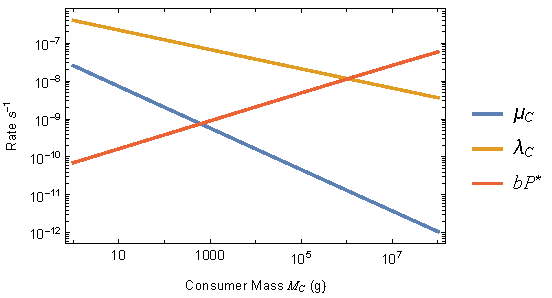
\includegraphics[width=0.7\textwidth]{../Figures/MortRateComparisonPlot.pdf}
  \caption{
	  An herbivore consumer's life-history mortality rate $\mu_C$, reproductive rate $\lambda_C$, and predation rate $bP^*$ as a function of its mass $M_C$ (g).
  }
  \label{fig:mortrate}
\end{figure*}

Even without exploring directly the consumer-resource dynamics, we can gain insight into the potential effects of predation mortality by comparing the mortality rate to the consumer's population growth rate $\lambda_C$ as a function of consumer mass $M_C$.
While the consumer's reproduction rate scales $\lambda_C \propto M^{-0.25}$, the predation mortality rate is shown to scale $bP^* \propto M^{0.37}$, meaning there is a consumer mass $M_C$ where these rates intersect.
For smaller consumer masses, the predation mortality rate is lower than the consumer's reproductive rate, suggesting that these populations can sustain a predator population.
However, as consumer mass increases, the predation mortality rate crosses $\lambda_C$, at which point the predation mortality rate becomes larger than the consumer reproductive rate.
This suggests that, given the optimal predator:prey mass scaling observed in diverse terrestrial communities (Eq. \ref{eq:opt}), there is a consumer mass threshold $M_C^{\rm crit}$ above which the consumer population can no longer sustain itself in the presence of such predative load.

While the analytical expression of $bP^*$ is not tractable, numerical assessment of this critical consumer mass gives $M_C^{\rm crit} = 1064$ Kg. 
Our analysis suggests that a consumer mass above this threshold cannot sustain a predator population with a predator:prey mass ratio observed for lower body masses, and with densities predicted by Damuth's Law.
Intriguingly, this corresponds to the body size of herbivores in the Serengeti that effectively escape predation due to their large size.
Cape buffalo have a mass $M_C \approx 450$ Kg, where predation accounts for roughly $23\%$ of mortality, whereas giraffes with  mass $M_C \approx 800$ Kg suffer $\approx 5\%$ mortality due to predation.
The next largest herbivore in the Serengeti are rhinoceros, which weigh $\approx 1200$ Kg and suffer $0 \%$ mortality due to predation (Sinclair et al.  2003), a threshold remarkably consistent with our estimated $M_C^{\rm crit}$ of 1064 Kg.

Previous efforts have evaluated the maximum sustainable terrestrial mammalian carnivore size to be roughly $700-1100$ Kg based on the energetic constraints of assimilated energy gain.
Here we provide an alternative perspective: that carnivore body size may be additionally limited by instabilities that the act of predation introduces to their herbivorous prey.
As our predicted allometric predator mortality rate crosses the consumer's reproductive rate at $M_C^{\rm crit}$, the populations of herbivore speciers larger than $1064$ Kg are expected to collapse, an effect that would be expected to cascade into the predator population.
Because we assume that predator mass is dependent on prey mass, we can estimate the predator mass that would destabilize its prey population, for which we obtain $M_P^{\rm crit} = 802$ Kg.
This estimate corresponds closely to the largest observed terrestrial apex carnivores: the Hyaenodontid \emph{Megistotherium osteothlastes} ranged between 500-800 Kg (Rasmussin 1989, Sorkin 2008), while the Oxyaenodont \emph{Sarkastodon mongoliensis} weighted $\approx 800$ Kg.
Other large mammalian predators are known to have existed, though their body mass is less well known due to a dearth of fossil specimens: \emph{Andrewsarchus} is famously thought to be the largest terrestrial predator ($800-1000$ Kg), while a recent skull of \emph{Smilodon populator} indicates that some individuals may have attained body sizes up to 900 Kg.

[Because our framework is constructed based on underlying energetic relationships, we can now ask: how do variations in less constrained model parameters alter these estimated mass thresholds?]
%We observe that the predicted thresholds are very sensitive to changes in the energy density of the consumer population.
%The above conditions assume reported energy densities of protein and fat, and that the consumable portion of the prey has a protein:fat ratio of $\approx 32:68$.
%If, however, the J/g of fat within consumable tissue is increased, so does its energy density, which would be the case for prey such as marine mammals.
%For example, if the J/g of fat within consumable tissue is increased by 5\%, we observe the threshold predator body size to increase to 795 Kg; if the J/g of fat is increased by 10\%, threshold predator mass increases to 1000 Kg.
%While we do not examine specifically the changed conditions of prey within maritime environments, the largest terrestrial carnivore \emph{Ursus maritimus} maintains a diet composed of the energy-rich marine mammals.
%The directionality of our model predictions thus affirms expectations of larger maximimum carnivore mass conditioned on a diet composed of prey with tissues that have greater energy density.

[Pleistocene implications]




\end{document}


